\documentclass[12pt, a4paper,twoside]{tesi_upf}

\usepackage[utf8]{inputenc}
\usepackage[T1]{fontenc}
\usepackage[spanish]{babel}
\usepackage[cam,a4,center,frame]{crop}
\usepackage{graphicx}
\usepackage{times}
\usepackage{url}
%\usepackage{natbib}
%\usepackage{garamond}
\pagestyle{plain}
\usepackage{bibentry}

\usepackage{float}
%\floatstyle{boxed}
%\restylefloat{figure}

\usepackage{amssymb}
\usepackage{amsmath}
\usepackage{listings}
\lstset{language=C++}

\usepackage{color}

\definecolor{mygreen}{rgb}{0,0.6,0}
\definecolor{mygray}{rgb}{0.5,0.5,0.5}
\definecolor{mymauve}{rgb}{0.58,0,0.82}


\lstset{ %
  backgroundcolor=\color{white},   % choose the background color; you must add \usepackage{color} or \usepackage{xcolor}
  basicstyle=\footnotesize,        % the size of the fonts that are used for the code
  breakatwhitespace=false,         % sets if automatic breaks should only happen at whitespace
  breaklines=true,                 % sets automatic line breaking
  captionpos=b,                    % sets the caption-position to bottom
  commentstyle=\color{mygreen},    % comment style
  deletekeywords={...},            % if you want to delete keywords from the given language
  escapeinside={\%*}{*)},          % if you want to add LaTeX within your code
  extendedchars=true,              % lets you use non-ASCII characters; for 8-bits encodings only, does not work with UTF-8
  frame=single,                    % adds a frame around the code
  keepspaces=true,                 % keeps spaces in text, useful for keeping indentation of code (possibly needs columns=flexible)
  keywordstyle=\color{blue},       % keyword style
  language=Octave,                 % the language of the code
  morekeywords={*,...},            % if you want to add more keywords to the set
  numbers=left,                    % where to put the line-numbers; possible values are (none, left, right)
  numbersep=5pt,                   % how far the line-numbers are from the code
  numberstyle=\tiny\color{mygray}, % the style that is used for the line-numbers
  rulecolor=\color{black},         % if not set, the frame-color may be changed on line-breaks within not-black text (e.g. comments (green here))
  showspaces=false,                % show spaces everywhere adding particular underscores; it overrides 'showstringspaces'
  showstringspaces=false,          % underline spaces within strings only
  showtabs=false,                  % show tabs within strings adding particular underscores
  stepnumber=2,                    % the step between two line-numbers. If it's 1, each line will be numbered
  stringstyle=\color{mymauve},     % string literal style
  tabsize=2,                       % sets default tabsize to 2 spaces
  title=\lstname                   % show the filename of files included with \lstinputlisting; also try caption instead of title
}

\usepackage{makeidx}
\makeindex

%BIBLIOGRAPHY STYLE
\bibliographystyle{apalike}


%LANGUAGE
\selectlanguage{spanish}

\addto\captionsspanish
  {\renewcommand{\contentsname}{\Large \sffamily Índice}}


%YOUR INFORMATION HERE:

\title{Implementación del algoritmo de path tracing en la GPU}
\subtitle{}
\author{Joaquim Romo}
\thyear{2014}
\department{GTI}
\supervisor{Javier Agenjo}

\includeonly{
	content/1_Introduccion,
	content/2_Fundamentos,
	content/3_Optix,
	content/4_Implementacion,
	content/5_Conclusiones
	%content/3-ResearchObjectives,
	%content/4-ResearchPlanAndMethodology,
	%content/5-SummaryOfPriorWork,
	%content/6-Significance
}

%\linespread{1.25}

\begin{document}


\frontmatter

\maketitle

\cleardoublepage




\selectlanguage{spanish}
\section*{\Large \sffamily Resumen}

El presente trabajo tiene como objetivo el estudio y la implementación de un algoritmo de renderizado con raytracing estocástico en la unidad de procesamiento de gráficos (GPU).
Se ha elegido realizar la implementación en una arquitectura de este tipo debido a las ventajas que ofrece en cuanto a tiempo de ejecución, gracias a la gran capacidad de cómputo en paralelo que ofrecen las arquitecturas de GPU actuales.


La primera parte del trabajo se dedica al estudio teórico del algoritmo de pathtracing, se comentan algunos conceptos físicos básicos relacionados con el transporte de luz y su interacción con los materiales así como las ecuaciones matemáticas y las técnicas estadísticas necesarias para la comprensión y correcta implementación del algoritmo.


En una segunda parte se discuten las tecnologías involucradas, concretamente el uso que se hace de la arquitectura CUDA, la librería OptiX y su funcionamiento y la implementación del algoritmo que se ha realizado sobre estas.  

%DIFFERENT TABLES OF CONTENT:

\tableofcontents
\listoffigures

\addcontentsline{toc}{chapter}{Índice de figuras}

\cleardoublepage

%HERE STARTS THE TEXT:
\mainmatter
\chapter{Introducción}

\section{Contexto}

En el entorno de la imagen generada por computador siempre ha sido un reto tratar de generar imágenes lo más realistas posibles. Para ello un gran número de investigadores se han dedicado a diseñar algoritmos que simulan o imiten el comportamiento y la interacción de la luz con los materiales. Estos algoritmos que tratan de simular de forma realista el comportamiento de la luz son generalmente conocidos como algoritmos de iluminación global.

Estos algoritmos, por lo general, suelen tener una complejidad computacional muy elevada y el tiempo de cómputo necesario para obtener un resultado satisfactorio en escenas complejas era un factor limitador en su aplicación práctica. Por ello las aplicaciones que hacen uso de gráficos 3D en tiempo real típicamente se centran en la iluminación local o directa de los objetos de la escena y simulan la iluminación indirecta mediante técnicas que aun sin tener un fundamento físico ofrecen una mayor credibilidad para el ojo humano. Estas técnicas suelen ser algoritmos de postprocesado que se aplican en espacio de pantalla, por ejemplo “ambient occlusion” o “directional occlusion”. 

Sin embargo en los últimos años se han realizado grandes avances en las arquitecturas de las unidades de procesamiento de gráficos (GPUs), en especial la gran capacidad de cómputo en paralelo debido al elevado número de microprocesadores que forman estos dispositivos. Con tal de aprovechar estos avances en el hardware, los fabricantes de GPU han desarrollado librerías de computo generico (OpenCL, CUDA) que ofrecen gran libertad al programador para implementar sus propios algoritmos.

Estas mejoras han permitido realizar implementaciones de algoritmos de iluminación global en las GPUs que son mucho más rápidos que las implementaciones típicas en la CPU permitiendo reducir el tiempo de cómputo de varias horas o días a minutos e incluso a ratios interactivos dependiendo de la GPU y algoritmos utilizados.

\clearpage

\section{Algoritmos de iluminación global}

Se conoce como algoritmos de iluminación global aquellos que tratan de simular distintos aspectos del comportamiento de la luz en su interacción con los objetos de una escena tridimensional. Algunos de ellos están pensados y optimizados para fenómenos concretos mientras que otros tratan de recrear fielmente todos los aspectos del transporte de luz.

En esta sección revisaremos por encima algunos de los algoritmos clásicos.

 
\subsection{Radiosity (Goral et al. 1984)}

Radiosity fue el primero de los algoritmos de iluminación global que se desarrollaron. Inicialmente el algoritmo fue desarrollado en los años 1950 para aplicarlo al problema de la transferencia de calor. En 1984 fue modificado y adaptado por Cindy M. Goral, Kenneth E. Torrance, Donald P. Greenberg y Bennett Battaile, investigadores de la universidad de Cornell para su aplicación en la generación de imagen sintética.

Este algoritmo trata de resolver el problema de la iluminación indirecta entre superficies puramente difusas o Lambertianas.


\chapter{Fundamentos teóricos}

\section{Unidades Radiométricas}
Se conoce como radiometría al estudio de las radiaciones electromagnéticas. Ya que la luz visible es una onda electromagnética los algoritmos de renderizado que buscan el realismo se fundamentan sobre conceptos radiométricos. Por ello en esta sección haremos una pequeña introducción sobre algunos conceptos básicos que nos permitirán entender mejor los algoritmos de iluminación global.  
\subsection{Flujo}

El flujo radiométrico mide la cantidad de energía radiante por unidad de tiempo. Sus unidades son Watts o Joules/segundo.

\begin{equation}
\Phi = \frac{dQ(t)}{dt}
\end{equation}

\subsection{Irradiancia}
La irradiancia representa el flujo incidente en una superficie y se mide como el flujo radiante por unidad de área y sus unidades son de $W/m^2$ 

\begin{equation}
E = \frac{d\Phi}{dA}
\end{equation}

\clearpage

\subsection{Angulo solido}
El angulo solido no es una unidad radiométrica en si mismo pero es un concepto geométrico necesario para poder explicar otros conceptos radiométricos además de otros apartados del presente trabajo.

Podemos entender el concepto de angulo solido como la extension del angulo a las tres dimensiones.
\begin{figure}[h]
\centering
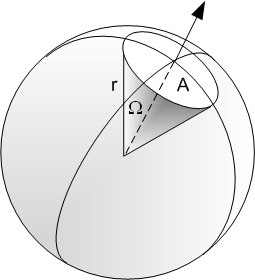
\includegraphics[width=2in]{Solid_Angle.png}
\caption{Definición de angulo solido \cite{Haade}}
\end{figure}

El angulo solido se mide como el área proyectada sobre una esfera de radio unitario. Sus unidades son adimensionales y son llamadas estereorradianes $[sr]$.
\begin{equation}
\Omega = \frac{A}{r^2}
\end{equation}


Usando coordenadas esféricas $\Theta = (\phi , \theta )$ podemos definir el angulo solido diferencial como:

\begin{equation}
d \omega _ \Theta = \sin \theta d \theta d \phi
\end{equation}

Informalmente resulta sencillo entender el angulo solido si pensamos en \emph{cuan grande se ve un objeto}. Supongamos una superficie perpendicular a la dirección de visión del observador: si este objeto esta muy cerca, diremos que subtiende un angulo solido mayor que la misma superficie a una mayor distancia en la misma dirección.

\clearpage

\subsection{Radiancia}

La radiancia, también llamada intensidad por algunos autores, es probablemente la unidad radiométrica mas importante en lo que concierne al presente trabajo y a muchos de los algoritmos de iluminación global ya que su valor es invariante a lo largo de la longitud de un rayo.

Esta unidad mide la irradiancia por unidad de angulo solido.

\begin{equation}
L = \frac{dE}{d\omega} = \frac{d^2\Phi}{d\omega dA\cos \theta} 
\end{equation}


\clearpage

\section{BRDF}

La función de distribución de reflectancia bidireccional (de ahora en adelante BRDF, por sus siglas en inglés), definida por primera vez por \cite{Nicodemus1965} Nicodemus (1965), es un función que define la respuesta a la luz de una superficie opaca, tomando como parámetros dos vectores unitarios que definen las direcciones de entrada y salida de la luz. Más formalmente, la BRDF mide la relación entre la radiancia diferencial reflejada en la dirección de salida y la irradiancia diferencial entrante en el ángulo sólido diferencial alrededor del vector de entrada

\begin{equation}
f(x, l, v)=\frac{dL(x \to v)}{dE(x \gets l)} = \frac{dL(x \to v)}{L(x \gets l) \cos\theta d\omega_i} 
\end{equation}

donde $l$ es el vector unitario que apunta en la dirección opuesta a la de entrada de la luz y $v$ es el vector unitario que apunta en la dirección de salida de la luz.

La BRDF solo esta definida para vectores $l$ y $v$ tales que $n \cdot v > 0, n \cdot l > 0$, siendo $n$ la normal de la superficie.

\begin{figure}[h]
\centering
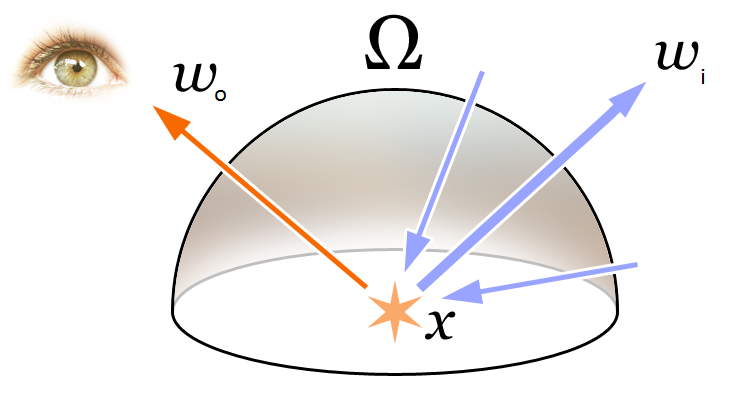
\includegraphics[scale=0.5]{Rendering_eq.png}
\caption{BRDF $l = \omega_i, v = \omega_o$ \cite{Timrb2008}}
\end{figure}


Para obtener la radiancia total reflejada en un punto $x$ en la dirección saliente $v$ es necesario integrar sobre el angulo solido en el dominio de la hemiesfera centrada en $x$.

\begin{equation}
\label{eq:radiance_integral}
L _ o = \int_{\Omega_x} f(x, l, v) L_i(l) (l \cdot n) d\omega_i 
\end{equation}

\clearpage

\subsection{Propiedades de la BRDF}

Una BRDF debe cumplir ciertas propiedades para que sea físicamente plausible.
En primer lugar debe cumplir la ley de conservación de la energía. En el caso que nos ocupa esto significa que una superficie puede absorber luz, transformándola en calor, o puede reflejarla pero en ningún caso puede reflejar mas energía lumínica que la que recibe.

\begin{equation}
\forall l, \int_{\Omega_x} f(x,l,v) (n \cdot v) d\omega_o \leq 1
\end{equation}

En términos informales esta ecuación significa que la integral de toda la luz reflejada debido a un rayo de luz entrante nunca podrá ser superior a la luz entrante por ese rayo.

\medskip
Además también debe cumplir el \emph{principio de reciprocidad de Helmholtz}, esto significa que si intercambiamos los vectores $l$ y $v$ su valor se mantiene. Este hecho cobra sentido si pensamos que la BRDF es una característica intrínseca de cada material y que al intercambiar los vectores $v$ y $l$ el angulo entre ellos sigue siendo el mismo.

\begin{equation}
f(x, l, v) = f(x, v, l)
\end{equation} 

\subsection{Isotropía y anisotropía de la BRDF}

Una BRDF isotropica es aquella en la que su valor se mantendrá constante si aplicamos la misma rotación a $v$ y a $l$ alrededor de la normal de la superficie. Por el contrario una BRDF anisotropia cambiara su valor dependido de la rotación de $v$ y $l$ alrededor de la normal.

\clearpage

\subsection{Modelo de Phong modificado}
Una de las BRDFs mas usadas en los algoritmos de ray tracing estocástico es la BRDF basada en el modelo de Phong modificado, que fue descrito por primera vez por Lewis (1994) \nocite{Lewis1994} y posteriormente explorado en mas profundidad en \cite{Lafortune1994}. Esta BRDF esta basado en el conocido modelo de reflexión local de Phong \cite{Phong1975} que fue adaptado por Lewis para cumplir con el principio de conservación de la energía.

En la forma usada por Lafortune y Willems la función aparece como:

\begin{equation}
f(x, l, v) = \frac{k_d}{\pi} + k_s \frac{n + 2}{2 \pi} \cos^n\alpha
\end{equation}

donde $\alpha$ es el angulo entre la dirección de reflexión especular perfecta y $l$.
En esta forma la función esta normalizada para conservar la energía pero además para que esto sea cierto se debe cumplir $k_d + k_s \leq 1$.



\clearpage

\section{Ecuación de renderizado}

La ecuación de renderizado fue desarrollada en los años 80 simultaneamente y de forma independiente por distintos autores \cite{Kajiya1986, Immel1986}. Se trata de una ecuación integral que unifica y formaliza los distintos algoritmos de renderizado, ya que hasta ese momento no existía un marco de trabajo teórico común.

\medskip
Existen varias versiones de esta ecuación, según el autor que la use, que en general se pueden clasificar en dos tipos: las que integran sobre la hemiesfera, que se corresponde con la ecuación propuesta por Immel y las que integran sobre la unión de las superficies de la escena, que es la version propuesta por Kajiya.
\medskip

Consideremos la ecuación \ref{eq:radiance_integral}  y consideremos que además de dispersar luz una superficie también puede emitir luz, siendo $L_e$ la radiancia de la luz emitida, entonces tenemos la ecuación de renderizado.

\begin{equation}
L _ o = L_e + \int_{\Omega_x} f(x, l, v) L_i(l) (l \cdot n) d\omega_i 
\end{equation}

Es decir, que la radiancia total $L_o$ que sale de un punto $x$ es igual a la suma de la radiancia emitida por ese punto en la dirección de salida $v$ mas la integral de toda la radiancia que llega a ese punto y es reflejada en la dirección de salida.
\medskip

Lo significativo de esta ecuación es que resulta muy intuitivo derivar algoritmos de renderizado de la misma: se evalúa para cada punto a pintar y se evalúa $L_i$ recursivamente hasta que se cumpla determinada condición.
\medskip

El problema es que no parece factible encontrar una solución analítica de esta ecuación y por este motivo se aplican métodos de integración numérica para aproximar una solución.

\clearpage

\section{El método de montecarlo}

El método de montecarlo se trata de un método de integración numérico para integrales definidas sobre un dominio de dimension arbitraria, del tipo:
\begin{equation}
I = \int_D f(x)dx , D \subseteq \mathbb{R}^m
\end{equation}

Sabemos que la esperanza de una función continua se define como la integral de la función por la probabilidad de $x$. Y que podemos estimar la esperanza calculando la media de los valores que toma la función en puntos aleatorios escogidos independientemente y con la misma distribución.

\begin{equation}
E(f(x)) = \int f(x)p(x)dx \approx \frac{1}{N} \sum _{i=1} ^N f(x_i) 
\end{equation}


El método de montecarlo se basa en este hecho para estimar el valor de una integral definida tomando muestras aleatorias sobre el dominio $x_1, x_2, ..., x_n \in D$ y aplicando:

\begin{equation}
\label{eq:montecarlo}
I = \int_D f(x)dx \approx \frac{1}{N} \sum _{i=1} ^N \frac{f(x_i)}{p(x_i)} 
\end{equation}

Siendo $p(x_i)$ la probabilidad de tomar una muestra $x_i$ concreta de entre todas las posibles en el dominio $D$. En el caso de tomar las muestras sobre una distribución uniforme en $D$:

\begin{equation}
\forall x_i, p(x_i) = \frac{1}{\int _D dx}
\end{equation}

\begin{equation}
I \approx \frac{\int _D dx}{N} \sum_{i=1} ^N f(x_i)
\end{equation}

El error en una estimación de este tipo se reduce a medida que $N$ crece.
\clearpage

\subsection{Muestreo de importancia}
    
Otra forma de reducir el error a parte de tomar mas muestras es tomarlas de forma mas inteligente. Anteriormente hemos supuesto que tomamos las muestras de una distribución uniforme sobre el dominio pero el método de montecarlo no impone ninguna limitación en este aspecto. Lo que implica que podemos tomar las muestras de otro tipo de distribuciones que sean mas apropiadas para cada caso. Por ejemplo tomando mas muestras en aquellas partes del dominio de integración que sean mas interesantes o importantes para nuestros propósitos.

\medskip

Para ello basta con tomar las muestras $x_1, x_2, ..., x_n$ según la distribución usada y substituir $p(x_i)$ en la ecuación \ref{eq:montecarlo} por la probabilidad correspondiente.

\subsection{Muestreo estratificado}

El muestreo estratificado es otro método para reducir la variancia de la estimación. En este caso lo que se hace es dividir el dominio de la integral en regiones y aplicar montecarlo para cada región. 

\clearpage

\section{Aplicaciones del muestreo de importancia}

En esta sección veremos dos aplicaciones practicas en los algoritmos de ray tracing estocástico del muestreo de importancia y como usando esta técnica es posible reducir el numero de muestras necesarias para obtener una buena estimación de la integral.


\subsection{Muestreo de la BRDF}
\label{muestreo_brdf}
Aunque algunos de los conceptos explicados aquí son aplicables a otros modelos, para esta explicación nos centraremos en la BRDF de Phong modificada, ya que es la usada en nuestra implementación además de una de las mas exploradas \cite{Lafortune1994}.



\medskip

El problema que nos ocupa se nos presenta cuando tenemos que estimar la luz que llega a un punto del espacio. Una aproximación \emph{naive}, sin usar muestreo de importancia, seria muestrear uniformemente direcciones en la hemiesfera y evaluar la BRDF para cada dirección. Esto puede funcionar bien cuando se trata de materiales puramente difusos, sin componente especular o con un lóbulo especular muy abierto. Por el contrario en el caso de encontrarnos con una superficie altamente especular, como por ejemplo un metal, la cantidad de muestras necesarias para obtener una estimación decente seria desorbitada ya que la probabilidad de elegir una dirección dentro del lóbulo especular seria muy pequeña.

\medskip
Cuando nos encontremos en la tesitura de tener que muestrear proporcionalmente a la BRDF lo primero que habrá que tener en cuenta sera decidir si muestrear la parte difusa o la parte especular de la BRDF de forma proporcional a las características del material en cuestión. Es decir que para un rayo, la probabilidad de muestrear el lóbulo difuso sera de $k_d$, la probabilidad de muestrear el lóbulo especular sera $k_s$ y la probabilidad de ser absorbido sera $1 - k_d - k_s$.

\medskip

Para ello generaremos un numero aleatorio $0 \leq r \leq 1$ y si
$r \leq k_s$ muestrearemos la parte especular,
si $k_s < r \leq k_s + k_d$ muestrearemos la parte difusa
y si $k_s + k_d < r$ el rayo sera absorbido por el material.

\medskip

Una vez decidido el evento a evaluar procederemos de forma distinta según cada caso. En el caso de evaluar la parte difusa podemos muestrear uniformente sobre la hemiesfera o podemos muestrear usando una distribución coseno como defienden algunos autores.

\clearpage

Una forma sencilla de obtener puntos distribuidos con densidad de coseno en la hemiesfera es generar puntos uniformemente sobre un circulo unitario y luego proyectarlos a la hemiesfera.
Para ello generamos dos números aleatorios $r_1$ y $r_2$ en el intervalo $[0, 1]$ y hacemos:

\smallskip

$x = r_1 \cos (2\pi r_2)$

\smallskip

$y = r_1 \sin (2\pi r_2)$

\smallskip

$z = \sqrt{1 - x^2 - y^2}$

\smallskip

$l = (x, y, z)$

\medskip

En este caso la funcion de densidad de probabilidad (pdf) es

\smallskip

\begin{equation}
pdf(l_{diff}) = \frac{(l \cdot n)}{\pi}
\end{equation}

La parte mas interesante es muestrear el lóbulo especular de la BRDF. Una buena explicación del procedimiento se encuentra en \cite{Lafortune1994}. En este caso la función de densidad de probabilidad es

\begin{equation}
pdf(l_{spec}) = \frac{n + 1}{2\pi}\cos^m\theta
\end{equation}

Siendo $\theta$ el angulo entre $l$ y el vector $R = -v + 2n(n \cdot v)$, es decir $v$ reflejado respecto a la normal, que es la dirección de reflexión especular perfecta. De este modo conseguiremos direcciones mas parecidas a $R$ cuanto mayor sea el exponente especular.

\medskip

El vector resultante de muestrear esta pdf, en coordenadas esféricas:

\begin{equation}
(\phi, \theta) = (2\pi r_1, \arccos(r_2^{\frac{1}{n+1}}) 
\end{equation}

En ambos casos se prosigue trazando el rayo con la dirección obtenida y se calcula la radiancia reflejada en la dirección $v$ en función de la radiancia entrante $L(x \gets l)$ del siguiente modo:
\medskip

si estamos evaluando el factor difuso
\begin{equation}
L(x \to v) = \frac{L(x \gets l)k_d(n \cdot l)}{q_1 pdf_{diff}(l)}
\end{equation}

si evaluamos el factor especular

\begin{equation}
L(x \to v) = \frac{L(x \gets l)k_s(n \cdot l)(R \cdot l)^n}{q_2 pdf_{spec}(l)}
\end{equation}
siendo $R$ el vector $v$ reflejado respecto a la normal.

si el rayo es absorbido la contribución es $0$.




\clearpage

\subsection{Muestreo del angulo solido subtendido}
\label{sample_solid}

Como en este trabajo estamos calculando la integral de la luz dispersada integrando la hemiesfera, cuando tengamos que muestrear un fuente de luz sera necesario integrar el angulo solido subtendido por dicha fuente de luz. A priori, no sabemos si la fuente de luz estará ocluida pero si que podemos saber que angulo subtiende con respecto al punto sobre el que estamos calculando la luz que llega, por lo tanto la idea sera lanzar solo rayos dentro de este angulo solido para que vayan dirigidos hacia la fuente de luz.

\medskip

Para proceder de este modo sera necesario calcular el angulo solido y definir una estrategia de muestreo para cada tipo de luz presente. En este trabajo hemos utilizado luces esféricas pero es posible aplicar un método similar para luces poligonales.

\subsubsection{Esfera}

Para el muestreo del angulo sólido subtendido por una luz esférica nos basaremos en el método propuesto en \cite{Shirley1996}.

\medskip

En primero lugar tenemos que calcular el angulo solido en relación al punto $x$ subtendido por una esfera de radio $r$ centrada en $c$. Llamaremos $\theta_{max}$ al angulo entre la dirección del vector $c - x$ y una recta tangente a la esfera que pasa por $x$. Entonces

\begin{equation}
\cos \theta_{max} = \sqrt{1 - \sin^2 \theta_{max}} = \sqrt{ 1 - \left(\frac{r}{\lVert c - x \rVert} \right)^2 }
\end{equation}

Según la definición de angulo solido el angulo solido subtendido por la esfera en $x$ es:

\begin{equation}
\omega_x = 2\pi (1 - cos \theta_{max})
\end{equation}

La función de densidad de probabilidad de muestrear una dirección cualquiera $l$ dentro del angulo sólido sera la inversa del angulo solido subtendido es decir $p(l) = \frac{1}{\omega_x}$.

\medskip

Para obtener direcciones dentro del angulo sólido $\omega_x$ generamos dos números aleatorios $r_1$ y $r_2$ uniformemente en el rango $[0, 1]$, la dirección en coordenadas esféricas sera:

\begin{equation}
(\theta, \phi) = (\arccos (1 + r_1 (\cos \theta_{max} - 1)), 2\pi r_2);
\end{equation}

\clearpage

Para obtener la dirección del vector $l$ en coordenadas absolutas creamos una base ortonormal $(u, v, w)$ con $w = \frac{c - x}{\lVert c - x \rVert}$ y multiplicamos la matriz de la base ortonormal por la representación en coordenadas cartesianas de la dirección que hemos obtenido.

\begin{equation}
l = \begin{pmatrix}
u_x & v_x & w_x \\
u_y & v_y & w_y \\
u_z & v_z & w_z
\end{pmatrix}
\begin{pmatrix}
\cos \phi \sin \theta \\
\sin \phi \sin \theta \\
\cos \theta
\end{pmatrix}
\end{equation}







\chapter{Introducción a OptiX}


OptiX es una librería desarrollada por Nvidia para hacer ray tracing en la GPU. OptiX fue desarrollada con el propósito de ser lo mas flexible posible y adaptarse a las necesidades del programador. Por ello solo ofrece la funcionalidad de lanzar rayos y es responsabilidad del programador implementar el funcionamiento de esos rayos: como serán lanzados, que datos portaran, que sucederá cuando intereseccionen con un objeto, etc.

\medskip

Esta funcionalidad se implementa mediante lo que en OptiX se llaman programas. Los programas de OptiX son fragmentos de código CUDA con acceso a las funciones de OptiX, básicamente para el trazado de rayos, que serán compilados por el compilador de Nvidia (nvcc) y se ensamblaran en kernels CUDA para ser ejecutados en la GPU. 

\medskip
De ahora en adelante cuando hablemos de programas nos estaremos refiriendo a estos fragmentos de codigo CUDA, cuando queramos referirnos al conjunto del sistema de renderizado que es el objeto de este trabajo usaremos la expresión aplicación o sistema. Además en el contexto de CUDA y OptiX se conoce como Device a la GPU y como Host a la CPU.

\clearpage

\section{Device}

OptiX tiene un conjunto de programas que pueden ser implementados. Cada uno de ellos se encarga de una tarea especifica dentro del flujo de ejecución de una aplicación OptiX. En esta sección veremos cuales son estos tipos de programas y que utilidad tiene cada uno de ellos.  

\subsection{Ray generation programs}

Este tipo de programas son los puntos de entrada de una aplicación OptiX y es desde donde se crear y lanzan los rayos primarios. Típicamente, en una aplicación de renderizado se implementa la cámara en un programa de esto tipo.

\subsection{Intersection programs}

Los programas de intersección se encargan de determinar si un rayo intersecciona con un objeto y en caso afirmativo retorna la distancia a la que se ha producido la intersección. Ademas, el programador tiene flexibilidad para calcular y retornar datos relativos a esta intersección, típicamente las coordenadas de textura, la normal a la superficie en el punto de intersección, etc.

\medskip

El hecho de que el programador pueda determinar si se ha producido una intersección ofrece gran flexibilidad para implementar distintos tipos de superficies, desde un simple triangulo o esfera a complejas superficies procedimentales.

\subsection{Bounding box programs}

Estos programas van ligados a los programas de intersección y su función es la de calcular una AABB (del inglés Axis Aligned Bounding Box) que contenga el objeto con el que están asociados. La implementación de estos programas no es obligatoria para que OptiX pueda determinar la intersección pero aceleran el proceso y son necesarios si se quiere construir una estructura de aceleración.

\subsection{Closest hit programs}

Este es el tipo de programa mas interesante para el caso que nos ocupa ya que aqui es donde se calcula el resultado final de una intersección, normalmente el color de un punto en el espacio. Aquí es donde se hacen los accesos a texturas, se hace el shading y se pueden lanzar rayos recursivamente.

\medskip

Estos programas, como su nombre indica, se ejecutan solo para la intersección mas cercana del rayo con la escena.

\subsection{Any hit programs}

Por el contrario, los programas any hit, se ejecutan para todas las intersecciones que encuentre un rayo en su camino, a menos que explicitamente se termine la ejecución del rayo.
Un uso típico de estos programas es para el calculo de sombras, si cualquier punto de la escena ocluye la luz se termina el rayo y se retorna este hecho. Lo cual ofrece un mayor rendimiento en contraposición a tener que esperar a encontrar la intersección mas cercana.

\subsection{Otros programas}

Los programas que hemos visto hasta ahora son los mas relevantes y los que ofrecen la mayoría de funcionalidades pero existen otros programas que se pueden implementar para ofrecer otras funcionalidad.

\clearpage

\section{Host}

Además de la parte del device que hemos visto hasta ahora, OptiX también ofrece una API en el host que sirve para encapsular y ensamblar todos los programas del device además de para hacer las transacciones de memoria entre el host y el device. Aunque la API de host es en lenguaje C, OptiX también proporciona un envoltorio de la misma en C++ que sera el que usaremos. 

\subsection{Clase Program}

La clase Program es la representación en lado host de los programas que iran al device.
Se crea una instancia de un Programa proporcionando una cadena de caracteres con el codigo del programa compilado o una ruta al fichero que contiene el codigo compilado. 

\subsection{Clase Geometry}

La clase geometry representa un objeto geometrico, se crea proporcionandole un Programa de intersección y un programa de bounding box.

\subsection{Clase Material}

Esta clase representa un el material de un objeto y puede contener un closest hit program y un any hit program.

\subsection{Clase GeometryInstance}

La clase GeometryInstance sirve para asociar crear una asociación entre una instancia de la clase Material y una instancia de la clase Geometry. Semanticamente lo que estamos haciendo al crear un GeomtryInstance es asociar un objeto geométrico de la escena con su material.

\subsection{Clase Context}

Una instancia de la clase context encapsula todos los datos necesarios para la ejecución de una aplicación optix, todos los objetos que hemos comentado anteriormente se ensamblan dentro de este y además el context contiene el programa de generación de rayos que sirve como punto de entrada. Cuando queramos realizar una ejecución de OptiX lo haremos a través del método launch del context.

\subsection{Buffers}

Ademas de las clases que hemos visto, OptiX también permite crear buffers para pasar datos de la memoria del sistema a la VRAM del device.


\chapter{Implementación}

En este capítulo analizaremos la implementación realizada de los conceptos teóricos vistos hasta ahora y el uso práctico de las tecnologías involucradas.

\medskip

El diseño de la aplicación está basado en el patrón de software \emph{facade} con la idea de ofrecer una interfaz en C++ de tipo librería de alto nivel, reutilizable y fácil de usar, que permita realizar renderizados realistas sin tener que preocuparse de los detalles de bajo nivel relativos a OptiX y CUDA, ni de todos los conceptos teóricos involucrados.

\medskip

Además sobre esta interfaz se ha construido un parser de escenas XML, para hacer aún más sencillo el acto de configurar y crear escenas.

\clearpage

\section{Interfaz de programación}

\subsection{Estructura TCamera}

Este tipo de datos representa la cámara de la escena y encapsula todos los datos relativos a la cámara. Para construir un objeto de este tipo le pasamos la posición de la cámara, la posición del objetivo y el ángulo de campo de visión.

\subsection{TSphereLight}

Esta estructura representa una luz esférica, tomando como parámetros la posición del centro de la esfera, su radio y una tripleta RGB representando su emisión de luz.

\subsection{TObjModel}

Es una estructura que representa un modelo 3D en formato .obj. Se construye pasándole la ruta del modelo. 

\subsection{Clase CPathtracer}

Este es el tipo de datos más relevante de nuestra interfaz. Todos los datos relativos a la escena y al renderizado son finalmente encapsulados en un objeto de este tipo. Una vez configurado, es el responsable de cargar los programás de OptiX y construir el \emph{Context} de OptiX y controlar la ejecución del mismo.

\subsection{Uso de la interfaz de programación}

Para explicar el funcionamiento de la interfaz lo haremos mediante un sencillo ejemplo que contiene las clases y métodos principales de la interfaz.

\definecolor{orange}{rgb}{1.0,0.5,0.2}
\definecolor{purple}{rgb}{0.5,0.2,0.9}
\definecolor{blue}{rgb}{0.0,0.0,0.8}
\definecolor{green}{rgb}{0,0.7,0}
\definecolor{black}{rgb}{0.0,0.0,0.0}

\lstdefinestyle{customc}{
  belowcaptionskip=1\baselineskip,
  breaklines=true,
  frame=L,
  language=C,
  showstringspaces=false,
  basicstyle=\footnotesize\ttfamily,
  keywordstyle=\bfseries\color{green},
  commentstyle=\itshape\color{purple},
  identifierstyle=\color{blue},
  stringstyle=\color{orange},
}


\lstset{style=customc}

\begin{lstlisting}
CPathtracer pt;

pt.setRenderSize(width, height);
pt.setSqrtSamplesPerPixel(sqrtspp);
pt.setBlockSize(200u);
pt.setMaxDepth(7);


pt.setCamera(TCamera(optix::make_float3(8.0, 9.0, 1.0), 
		optix::make_float3(7.0, 9.0, 0.5), 60.0f));
pt.addObjModel(
		TObjModel("assets/dabrovic-sponza/sponza.obj"));
pt.addLight(TSphereLight(optix::make_float3(2.0f, 2.0f, 2.0f),
		optix::make_float3(0.0f, 5.0f, 0.0f), 1.0f));

pt.prepare();
pt.renderAllSamples();
pt.saveToTGA("render_sponza.tga");
\end{lstlisting}

Este ejemplo sirve para ilustrar el funcionamiento de la interfaz con el motor de renderizado.
Veamos el funcionamiento de este ejemplo:
En primer lugar creamos una instancia de la clase CPathtracer para seguidamente especificar las dimensiones, en pixeles, de la imagen que vamos a renderizar usando el método \emph{void setRenderSize(unsigned int width, unsigned int height)}. 

\medskip

Seguidamente usamos la instrucción \emph{pt.setSqrtSamplesPerPixel(sqrtspp} para especificar el número de muestras por pixel. El valor que toma este método es la raíz cuadrada del número de muestras. Lo hacemos de este modo para asegurarnos de que la división de cada pixel se hará en regiones uniformes, dividiendo el pixel en \emph{sqrtspp} filas y \emph{sqrtspp} columnas.

\medskip

En la siguiente línea, especificamos un tamaño aproximado de los bloques en los que dividiremos la imagen. Entraremos en más detalle sobre este comportamiento en las secciones siguientes, pero de momento quedémonos con la idea de que la instrucción \emph{pt.setBlockSize(200u);} le dice al renderizador que debe dividir la imagen en bloques de aproximadamente 200x200 pixels. 

\medskip

A continuación especificamos la profundidad de recursión máxima. Este valor equivale al número de veces que un rayo rebotará por la escena antes de ser terminado. Hay que calibrar bien este valor, ya que un valor muy bajo produciría una iluminación pobre de la escena y un valor demasiado alto incrementaría el tiempo de ejecución innecesariamente.

\medskip

Seguidamente le pasamos al pathtracer un objeto de tipo TCamara inicializado con los valores de posición, objetivo y ángulo de visión deseado. Sólo puede haber una cámara activa a la vez por lo que la clase CPathtracer siempre usará la última que le especifiquemos.

\medskip

Los métodos \emph{addObjModel} y \emph{addLight} añaden modelos .obj y luces a la escena. A diferencia de la cámara, podemos llamar a estos métodos tantas veces como queramos para añadir luces y geometría a la escena.

\medskip

El método \emph{prepare} toma todos los datos de configuración que hemos especificado anteriormente y los compila en un \emph{Context} de OptiX para poder empezar el proceso de renderizado.

\medskip

Usamos la instrucción \emph{pt.renderAllSamples()} para efectuar un renderizado completo, de la imagen que tomará tantas muestras como hayamos especificado, y por último guardamos el resultado en una fichero TGA. Por simplicidad en este ejemplo hemos usado el método \emph{renderAllSample}, pero también existe la opción de renderizar sólo una muestra por pixel por llamada con el método \emph{void renderNextSample()}. Este método será útil cuando queramos dar un feedback visual del progreso del renderizado, calculando una muestra y pintando en pantalla el resultado cada vez.

\clearpage

\section{Renderizado por bloques}

Durante el proceso de implementación nos encontramos con una dificultad cuando se trataba de renderizar escenas con muchos polígonos: el sistema operativo impone un límite al tiempo de ejecución de una llamada a la GPU de unos pocos segundos. Si llamábamos a la ejecución de un Context de OptiX contra toda la imagen, es decir con tantos CUDA threads como pixels, el sistema operativo paraba la ejecución antes de que esta terminara.

\medskip

La solución que encontramos fue dividir la imagen en bloques de menor tamaño y lanzar una ejecución del Context para cada uno de estos bloques. Es como pintar varias imágenes de menor tamaño y luego juntarlas, con la diferencia de que mantenemos un buffer en la memoria del device, del tamaño de la imagen final, para no tener que hacer transacciones de memoria entre el host y el device ya que esto reduciría notablemente el rendimiento.

\clearpage

\section{Cámara}

\subsection{Host}

En el host precalculamos los datos de la cámara que serán constantes durante la ejecución: los vectores de la base ortonormal del sistema de coordenadas de cámara (front, left, up) y la relación (viewd) entre el vector front y el vector up en función del ángulo de visión fov.

\begin{lstlisting}
TCamera::TCamera(optix::float3 aposition, optix::float3 atarget, float afov)
{
	is_ok = false;
	if(afov <= 0.0f || afov >= 179.0f) return;

	position = aposition;
	target = atarget;
	fov = afov;
	viewd = 0.0f;

	front = optix::normalize(target - position);
	left = optix::normalize(optix::cross(optix::make_float3(0.0f, 1.0f, 0.0f), front));
	up = optix::normalize(optix::cross(front, left));

	viewd = 1.0 / tanf( fov * 0.5f * DEG2RAD);
	is_ok = true;		
}
\end{lstlisting}

\clearpage

\subsection{Device}

En el device tenemos un programa encargado de generar los rayos primarios que se lanzaran desde la cámara, para ello se le pasan desde el host una serie de parámetros necesarios para lanzar el rayo correcto.

\begin{lstlisting}
float2 offset = make_float2(offset_x, offset_y);
float2 startSample = make_float2(launch_index) + offset 
	+ make_float2(
	(float)(currentSample%sqrtspp) * (1.0f/(float)sqrtspp),
	(float)(currentSample/sqrtspp) * (1.0f/(float)sqrtspp)
);

float2 centerSample = make_float2(1.0f/float(2 * sqrtspp));
float2 d = (startSample + centerSample) / make_float2(screen_dim.x, screen_dim.y) * 2.f - 1.f;

d.x *= aspect_ratio;
float3 ray_origin = eye;
float3 ray_direction = normalize(d.x*U + d.y*V + W*viewd);
\end{lstlisting}

El offset son las coordenadas absolutas en espacio de imagen del pixel top-left del bloque que estamos pintando y el launch\_index es él índice del CUDA thread actual que se corresponde con las coordenadas relativas al bloque actual del pixel que estamos pintando. Usamos estas variables para calcular las coordenadas top-left del pixel que estamos pintando, en coordenadas absolutas de la imagen entera.

\medskip

Para que el muestreo múltiple de cada pixel proporcione antialiasing es necesario dividir el pixel en regiones y lanzar el rayo a través de la región que se corresponde con la muestra actual. Para calcular las coordenadas de la región actual lo hacemos a partir del parámetro currentSample y de la raíz cuadrada del total de muestras (la variable sqrtspp).

\medskip

Efectuados estos cálculos tenemos las coordenadas top-left absolutas de la región de pixel. A estas coordenadas le sumamos el valor de media región de pixel para que el rayo salga por el centro de dicha región, en vez de por su esquina superior-izquierda.

\medskip

En la variable d normalizamos esas coordenadas para obtener las coordenadas de pantalla correctas en el intervalo $[-1, 1]$. Corregimos la relación de aspecto de la imagen y calculamos la dirección del rayo resultante.

\clearpage

\section{Muestreo de la BRDF}

Para el muestreo de la BRDF usamos el modelo propuesto en \cite{Lafortune1994} que hemos explicado en la sección \ref{muestreo_brdf}.
\medskip

En primer lugar decidimos aleatoriamente si muestrear la parte difusa o la parte especular de la BRDF. Para ello proponemos usar como probabilidades las medias de los valores RGB de las componentes difusa y especular: $p_{diff} =\frac{1}{3}( k_{dR} + k_{dG} + k_{dB})$ y $p_{spec} =\frac{1}{3}( k_{sR} + k_{sG} + k_{sB})$ 

\medskip

Generamos un un número aleatorio $r$ en $[0,1]$ y si $r \leq p_{spec}$ muestreamos la parte especular, si $p_{spec} < r \leq p_{spec} + p_{diff}$ la parte difusa, en caso contrario el rayo es absorbido y terminamos la recursión del mismo.

\medskip

Esta forma de terminar la recursión se conoce como ruleta rusa y es una técnica de reducción de la varianza usado en integraciones por Montecarlo. Para compensar esta terminación anticipada y la separación entre rayos difusos y especulares, dividiremos el resultado entre la probabilidad de que se lance ese rayo. Ya que se muestrea con más probabilidad el evento más probable esto servirá para dar más peso a aquellas muestras menos probables.

\subsection{Muestreo de la parte difusa de la BRDF}
En el programa de closest hit, muestreamos la hemiesfera centrada en el punto de intersección para tener una estimación de la luz incidente.

\begin{lstlisting}
	unsigned int seed = prd_radiance.seed;
	float r1 = rnd(seed);
	float r2 = rnd(seed);
	float3 p;
	cosine_sample_hemisphere(r1, r2, p);
	
	float3 u, v;
	createONB(ffnormal, u, v);
	float3 rd = normalize(u * p.x + v * p.y + ffnormal * p.z);
		
	PerRayData_radiance diffuse_refl_prd;
	diffuse_refl_prd.seed = seed;
	diffuse_refl_prd.depth = prd_radiance.depth + 1;
	diffuse_refl_prd.contribution *= Kd;
	diffuse_refl_prd.is_light = false;
	optix::Ray diffuse_refl_ray( hit, rd, radiance_ray_type, scene_epsilon );
	rtTrace(top_object, diffuse_refl_ray, diffuse_refl_prd);
	brdfLight = diffuse_refl_prd.result;
	color += brdfLight * Kd / prob_diff;
\end{lstlisting}

Básicamente lo que hace es, en el caso de que no hayamos llegado a la profundidad de recursión máxima, muestrear un punto en la hemiesfera con densidad de coseno, generar una base ortonormal en función de la normal de la superficie y transformar el punto de la hemiesfera con esa base. Se traza un rayo recursivamente en la dirección obtenida y el color devuelto por ese rayo se multiplica por el color difuso de la superficie.

\medskip

Hay que hacer notar que en la instrucción \emph{color += brdfLight * Kd / prob\_diff;} no estamos multiplicando por el típico factor coseno de la normal y la luz. No lo hacemos porque al tomar la muestra con densidad coseno y dividir entre la densidad de probabilidad de esa muestra los factores coseno se anulan.
Siguiendo con ese razonamiento y teniendo en cuenta que la densidad coseno es $\frac{cos(l,n)}{\pi}$ deberíamos multiplicar el resultado por $\pi$ para ser coherentes con la teoría, pero lo hemos quitado del cálculo porque hemos comprobado empíricamente que el resultado final es más satisfactorio sin ese factor, que en caso de incluirlo en el cálculo generaba imágenes excesivamente iluminadas y quemadas.

\medskip

Usando solamente esta función de iluminación ya es posible generar renderizados, aunque al no muestrear las luces directamente tardarán más en converger.
En las primeras fases de la implementación realizamos algunos renderizados con este closest hit program, y un closest hit program para las fuentes de luz que devolvía su emisión de luz. Un ejemplo de ello puede verse en la siguiente figura.


\begin{figure}[h]
\centering
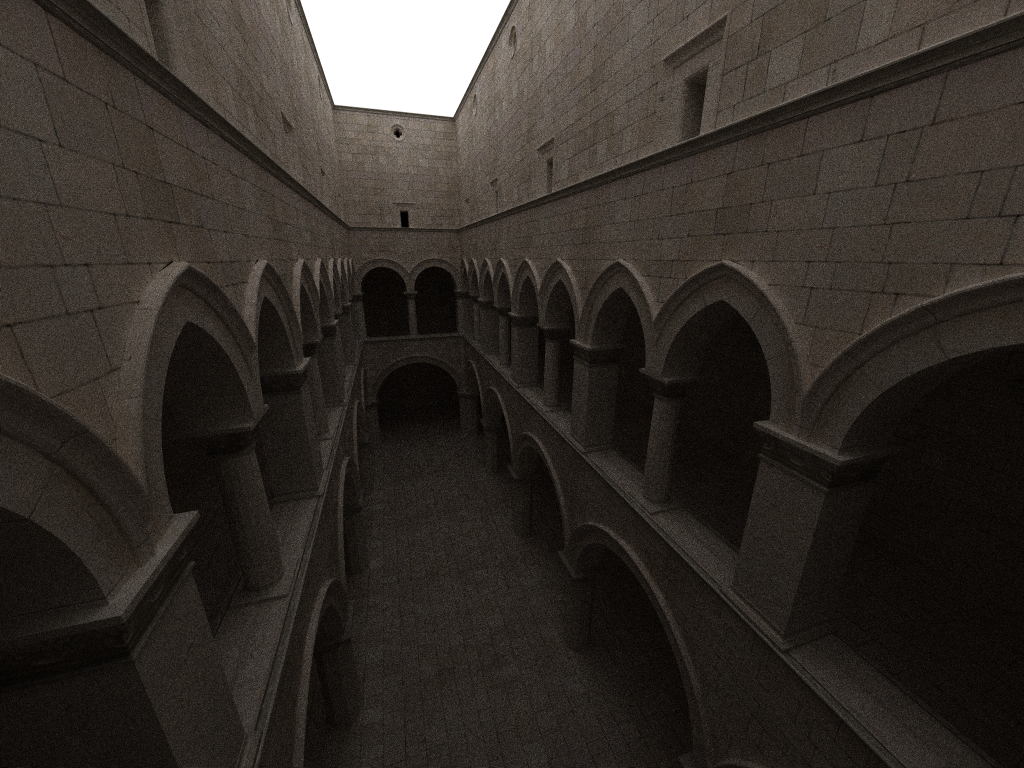
\includegraphics[width=5in]{dome1.png}
\caption{Muestreo de la brdf difusa}
\end{figure}

\clearpage

\subsection{Muestreo de la parte especular de la BRDF}

En el caso de la parte especular usamos como densidad de probabilidad una potencia de coseno de forma que el exponente sea mayor cuanto más reflectante sea el material. Ese vector es posteriormente transformado con una base ortonormal orientada hacia la dirección de reflexión perfecta.

\begin{lstlisting}
	float3 eye = -ray.direction;
	float3 perfect_specular = normalize(2.0 * ffnormal * dot(ffnormal, eye) - eye);
	createONB(perfect_specular, u, v);
	p = sample_specular2(phong_exp, r1, r2);
	float3 rd = normalize(u * p.x + v * p.y + perfect_specular * p.z);
	if(dot(rd, ffnormal) > 0.0f){
		PerRayData_radiance specular_refl_prd;
		specular_refl_prd.seed = seed;
		specular_refl_prd.depth = prd_radiance.depth + 1;
		specular_refl_prd.contribution *= Ks;
		specular_refl_prd.is_light = false;
		optix::Ray specular_refl_ray( hit, rd, radiance_ray_type, scene_epsilon );
		rtTrace(top_object, specular_refl_ray, specular_refl_prd);
		brdfLight = specular_refl_prd.result;
				
		color += ( brdfLight * Ks * (phong_exp + 2) * dot(rd, ffnormal) ) / ( (phong_exp + 1) * prob_spec );
	}

\end{lstlisting}

La función \emph{sample\_specular2} genera una dirección aleatoria con una densidad de probabilidad que depende del exponente especular, tal como hemos visto en la sección \ref{muestreo_brdf}.

\begin{figure}
\centering
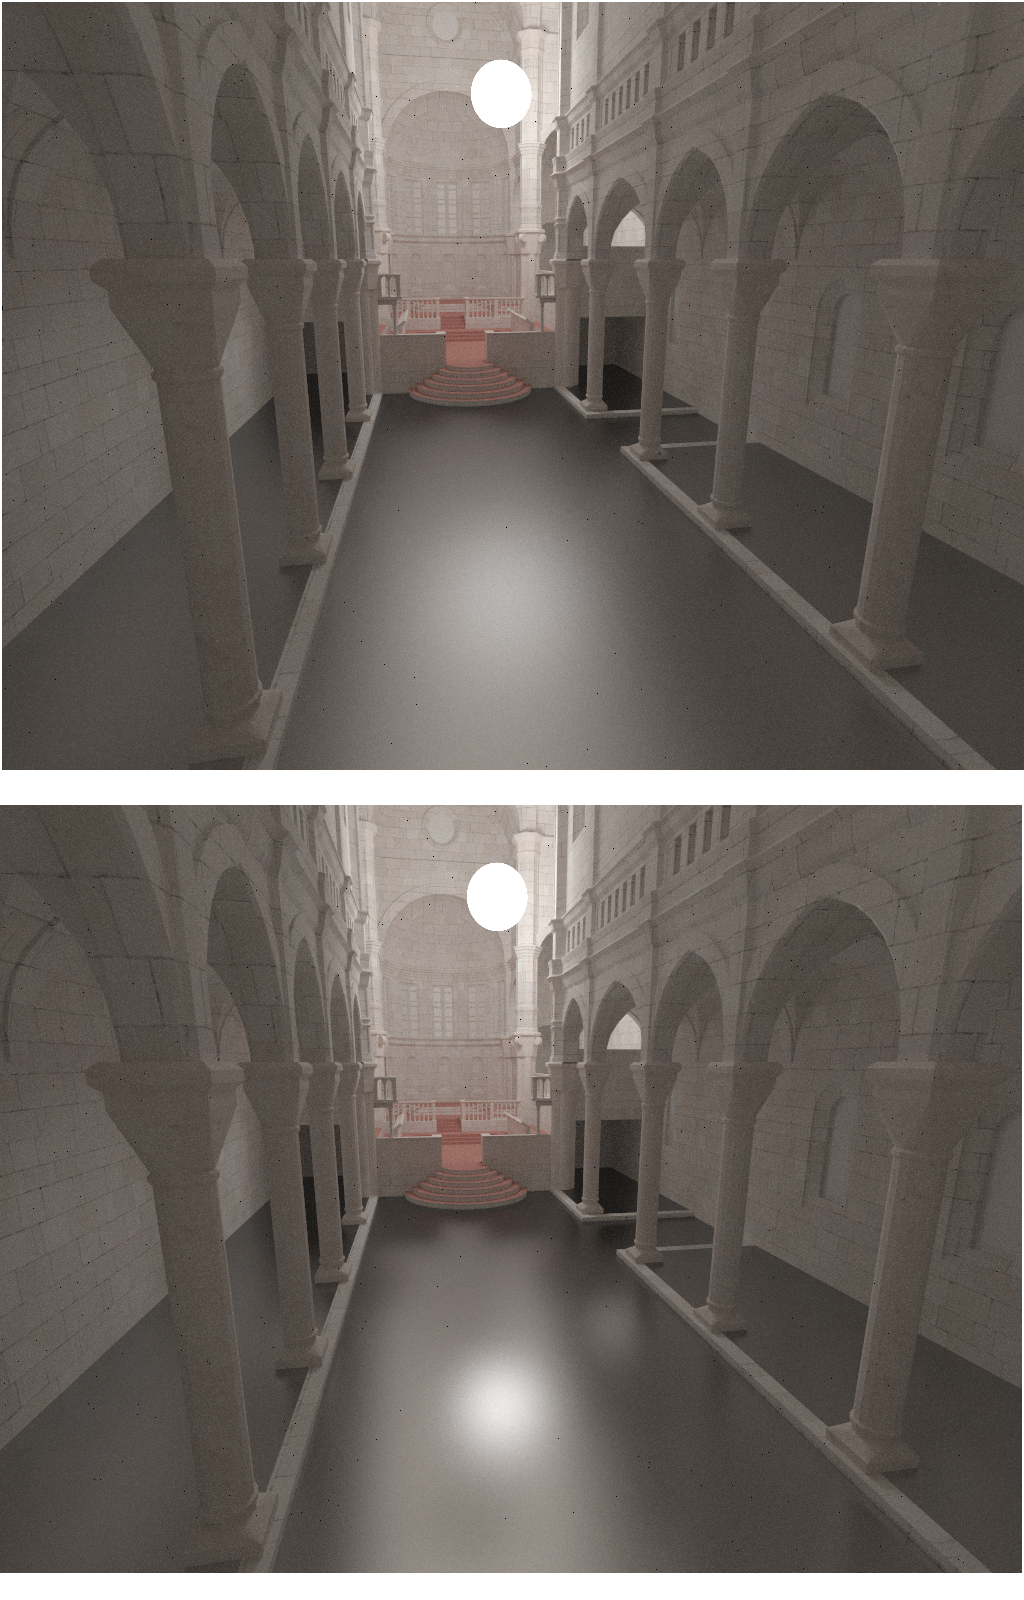
\includegraphics[width=5in]{compare_specular2_burned.png}
\caption{Arriba exponente especular de 64, abajo exponente de 512. Se puede apreciar que cuanto mayor sea el exponente más reflectante será el material.}
\end{figure}

\clearpage

\section{Muestreo de luces}

Una mejora importante que hemos implementado ha sido el muestreo directo de fuentes de luz. Muestrear las luces directamente provoca que el renderizado converja más rápido al lanzar rayos hacia zonas de la escena que es más probable que aporten luz al cómputo final.

\begin{lstlisting}

for(int i = 0; i < spherical_lights.size(); ++i){
	float3 light_dir = spherical_lights[i].center - hit;
	float dist2 = dot(light_dir, light_dir);
	float radius2 = spherical_lights[i].radius * spherical_lights[i].radius;
	if(dist2 - radius2 < scene_epsilon){
		continue;
	}
	unsigned int seed = prd_radiance.seed;
	float cos_theta_max = sqrtf(1 - radius2/dist2);
	float inv_pdf = 2.0f * PI * (1.0f - cos_theta_max);
	
	float r1 = rnd(seed);
	float r2 = rnd(seed);
	float cos_theta = 1 + r1 * (cos_theta_max - 1);
	float sin2theta = 1 - cos_theta * cos_theta;
	float sin_theta = sqrtf(sin2theta);
	float sin_phi = sinf(2 * PI * r2);
	float cos_phi = cosf(2 * PI * r2);
	float3 w = normalize(light_dir);
	float3 u, v;
	createONB(w, u, v);
	float3 dir = normalize( u * cos_phi * sin_theta + v * sin_phi * sin_theta + w * cos_theta );

	if(dot(dir, ffnormal) < 0) continue;
	PerRayData_shadow shadow_prd;
	shadow_prd.contribution = spherical_lights[i].emission;
	float delta = sqrtf(radius2 - sin2theta * dist2);
	Ray shadow_ray = Ray( hit, dir, shadow_ray_type, scene_epsilon, cos_theta * length(light_dir) - delta );
	rtTrace(top_object, shadow_ray, shadow_prd);
	color += inv_pdf * shadow_prd.contribution * dot(dir, ffnormal) * (Kd + Ks * powf(fmaxf(dot(dir, perfect_specular), 0.0f), phong_exp) );

}
\end{lstlisting}

Para cada luz esférica calculamos la distancia del punto que estamos evaluando al centro de la esfera y en caso de encontrarnos dentro de la misma la omitimos y continuamos con la siguiente.

\medskip


A continuación procedemos a generar una dirección dentro del ángulo sólido subtendido por la esfera, tal como se ha explicado en la sección \ref{sample_solid}. Si dicha dirección forma un ángulo superior a noventa grados con respecto a la normal la omitimos.

\begin{figure}[h]
\centering
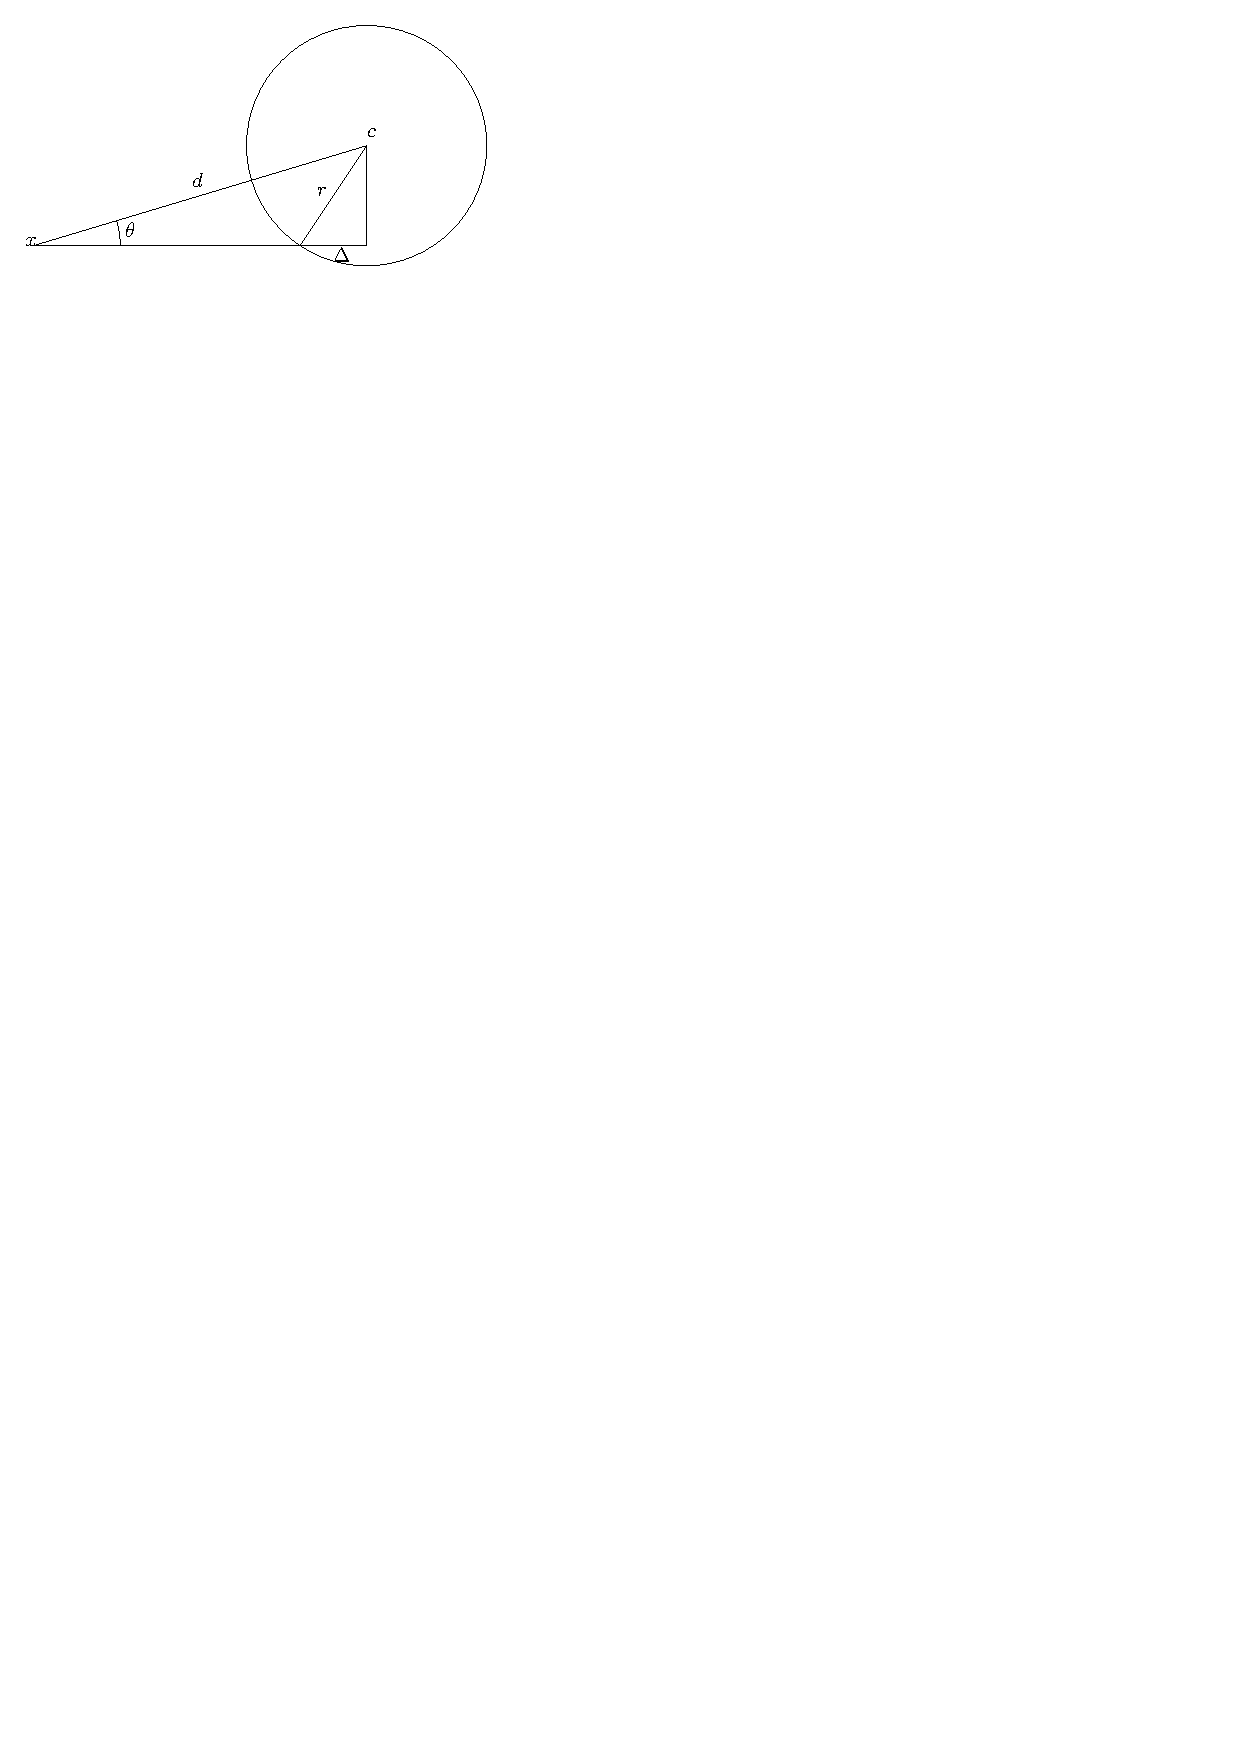
\includegraphics[scale=1.0]{sample_esfera.pdf}
\caption{  $\Delta $ al punto de intersección}
\end{figure}

La distancia a la que se encuentra el primer punto de intersección de la esfera con el rayo será $d_{intersect} = d \cos\theta - \Delta $. Este valor $\Delta = \sqrt{r^2 - (d\sin\theta)^2}$ lo calculamos en la instrucción \emph{float delta = sqrtf(radius2 - sin2theta * dist2);}. De este modo cuando creemos el rayo lo haremos con una distancia máxima que es la que nos interesa con tal de que no interseccione con objetos que estén dentro o detrás de la esfera. En las líneas 29 y 30 creamos y lanzamos el rayo. El valor \emph{shadow\_prd.contribution} será la emisión de luz de la fuente que estamos muestreando o $0$ si ha interseccionado con algún objeto.

\medskip

Finalmente en la última línea calculamos la contribución de luz de la muestra evaluando la BRDF.


\begin{figure}
\centering
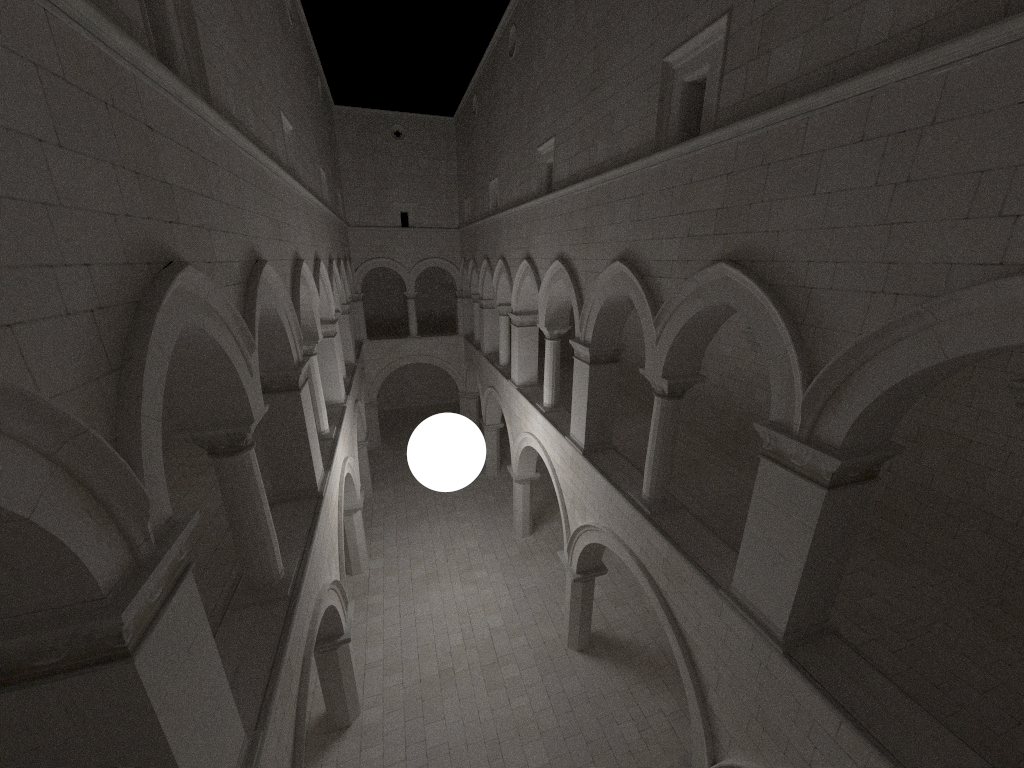
\includegraphics[width=5in]{esferica.png}
\caption{Fuente de luz esférica}
\end{figure}



\chapter{Conclusiones y resultados}


\section{Valoración de los resultados obtenidos}


El campo de estudio en el que se sitúa el presente trabajo es muy amplio y ha sido muy estudiado por un gran numero de investigadores. A medida que profundizábamos en la materia de estudio iban surgiendo cada ves mas detalles, mejoras y variaciones en la teoría que incrementaban el abasto del proyecto y generaban nuevas dudas. Por ello hemos llegado a un punto en el que, por el abasto de un TFG, hemos tenido que empezar a descartar cosas que al autor le hubiese gustado investigar en mas profundidad. Aun así, valoramos positivamente los resultados obtenidos pues se ha alcanzado el objetivo principal de este trabajo que era implementar un algoritmo de renderizado realista. Además la implementación en la GPU ha demostrado ser bastante rápida, mas aun si consideramos que la GPU usada en el desarrollo de este trabajo y en las pruebas realizadas es de una gama baja entre las presentes en el mercado.

\section{Posibles mejoras}

Planteamos tres grupos de posibles mejores bien diferenciados: En primer lugar tenemos las mejoras al algoritmo usado. El algoritmo de path tracing que hemos implementado es una de sus versiones mas basicas y tal como hemos comentado en la introducción existen variaciones del mismo que ofrecen mejores resultados en un menor numero de muestras. Por ejemplo, una primera mejora seria implementar el transporte de luz bidireccional que ofrecería mejores resultados cuando se trata de iluminar escenas en las que la fuente de luz esta muy escondida con respecto a la zona enfocada por la cámara. Otra importante mejora seria explorar e implementar modelos de BRDFs mas realistas, pues el que hemos usado es de los mas básicos que hay. Además, en este trabajo hemos omitido el importante fenómeno de la refractancia de la luz.

\medskip

Otro grupo de mejoras, mas allá de este algoritmo en concreto, seria buscar formas de combinar distintos algoritmos. Aunque en principio el algoritmo utilizado es capaz de simular los fenómenos de la luz mas habituales esto no significa que sea el mejor para todos ellos. Existen algoritmos que destacan en simular aspectos específicos del transporte lumínico y un buen motor de renderizado puede aprovechar ese hecho para combinar algoritmos de forma inteligente. Por ejemplo, versiones del algoritmo de radiosity o instant radiosity pueden usarse en una primera fase para computar un mapa de luz difusa de la escena. En una segunda fase se puede utilizar alguna de las variantes de path tracing para calcular la luz especular y la luz refractada, haciendo consultas al mapa de luz difusa cuando sea necesario. Finalmente una ejecución de photon mapping puede usarse para calcular las causticas con un mayor nivel de detalle.
Una buena explicación de este uso combinado de algoritmos se puede encontrar en \cite{Hery2013}.

\medskip

Por ultimo y aunque no era el objetivo de este proyecto, una mejora interesante seria implementar una interfaz de usuario que permitiese configurar la escena de forma fácil y cómoda. Por ejemplo una interfaz con Qt con una vista OpenGL, que permita previsualizar la escena, cargar modelos tridimensionales y colocar las luces y la cámara facilitaría mucho el hecho de configurar escenas y crear nuevos renderizados.


\section{Perspectivas de futuro}

Teniendo en cuenta los resultados obtenido, que la GPU utilizada no es de las del mejores del mercado y que nuestra implementación es muy optimizable. Considerando además la velocidad a la que avanza la tecnología de las tarjetas gráficas y que ya existen aproximaciones a soluciones de iluminación global con tiempos de renderizado interactivos, creemos que en pocos años sera habitual disponer de aplicaciones que hagan uso de este tipo de algoritmos en tiempo real. 


%\chapter{Research objectives}

UbiCALab.


\section{A Section}

UbiCALab.

\begin{table}[h]
  \centering
  \begin{tabular}{|l|l|}
   \hline
    0 & 0 \\ \hline
    0 & 0 \\ \hline    
  \end{tabular}
  \caption{Prova de taula}

\end{table}

\subsection{A Subsection}

UbiCALab.

\section{Another Section}

UbiCALab.. 

Incorpora una figura amb el logo de la UPF (Figura \ref{fig:logo}) {perque surti a l'index de figures. 
\begin{figure}[h]
  \centering
  
\includegraphics[scale=.5]{logo_upf.png}
    \caption{Exemple de grafic}
    \label{fig:logo}
\end{figure}

%\chapter{Research plan and methodology}

Lorem ipsum dicam tation maiorum vel ea, an nam minimum pertinax vituperatoribus, mea no illud tibique nostrum. Odio aperiri dolorem in sit, utinam labore adipiscing cu vel. Nam porro choro cu, nam virtute maluisset voluptatum in, per te vero iuvaret praesent. Eos ut volumus pertinacia interesset, tota debitis abhorreant mei et, clita electram pri at. Ea fabulas admodum theophrastus sea, id nostro omnium periculis sed. Vim id nulla aliquando. Id mel habeo nostrud mandamus, laudem legimus fastidii quo ea, ut iriure utamur quo.

Cu sit nobis omnesque scripserit, nec albucius perfecto salutatus ex. Novum debet propriae vis cu, sed ea suscipit accusata, nam minim salutandi voluptatum ut. Quaerendum definitiones est ut, no quo postea prompta scaevola. Nec at choro soleat causae, per ut docendi denique, discere veritus no sed. Ei sed sale delicatissimi mediocritatem, eligendi deterruisset ut mei, ignota offendit ocurreret at mel. Numquam blandit gubergren an pro, mei cu quot dolore recteque. Suscipit aliquyam principes eam ut, id error dicit perpetua qui.

Eam mentitum noluisse instructior cu, ad scripta nonummy aliquyam eos. Augue possit gloriatur mel an, mea et dolorum suavitate assueverit. At ius dolores persecuti moderatius, id qui justo tantas dissentiet. Integre invenire imperdiet ut mea, harum alienum officiis te nam, integre qualisque conceptam in vis. Viderer consetetur vim id, sumo tempor complectitur vim an. His te aeterno tamquam integre, nec agam aliquando repudiandae id, te fabellas verterem sea.

Per dicit veniam delicata ut, dicunt corpora mei eu. His no alienum accusata accommodare, eu nam clita audire invidunt. Mutat debitis mediocrem duo te, ex vis prima labore inermis. Usu eu dictas possim vocent. Suas meliore ancillae ad eum, eam ei cibo viderer similique.

Usu ne apeirian deserunt expetendis, sed in iisque abhorreant definiebas, quo nulla inermis appareat cu. Ei nam possim docendi pertinax, ut duis veritus detracto pri. Animal percipit ius ne, ne iisque quaeque philosophia pro, ut sed nobis nullam adolescens. Persius principes omittantur per an. Mel quot nostrud labores at, ad vis latine persius petentium. Cum partiendo neglegentur mediocritatem ut, per simul aliquando tincidunt no, falli nominavi molestiae ex nam.

Saperet inciderint in vim, vis quod civibus accusata in. Et ullum facilisi accommodare nec, decore utroque definitionem an vel, id duo kasd facer latine. Ea sumo ullamcorper per, ex pro nobis efficiendi concludaturque, vix eu verear luptatum ocurreret. Ocurreret intellegat te eum, ius ea cibo epicurei dignissim. Diam elit quaeque cum ut. Est dicat summo prodesset te, no vel harum saepe sensibus, et ignota altera doming qui.

Sit altera regione feugiat in, vim ad augue mediocritatem, duo reque choro theophrastus ea. Ipsum apeirian voluptatum duo no, nam ut ornatus accumsan percipitur, est no posse suscipiantur vituperatoribus. Errem legendos partiendo est cu, est clita signiferumque cu. Ea nulla scripta signiferumque eam, sea vidit dolores officiis ei, nibh saepe in nam. Ad vim justo dolor reprimique, eum ad labitur dissentias scriptorem, cu tempor mentitum assentior eum. Id vis mucius percipit invidunt.

Vel at ullum intellegam constituam, mea dicta affert perpetua ea. Eripuit blandit iracundia nec ea, tale timeam molestie cum te. Cum ei kasd mazim, per ei delenit ullamcorper, ad sale vocibus temporibus usu. An nonummy oporteat phaedrum sed, eu unum deserunt incorrupte mei. His an possim delicata, ei accumsan constituam mea. Ei viris constituam pro, cu inimicus argumentum duo.

Cu regione veritus persequeris vis, tation nusquam percipit in pri, vis no labitur deseruisse. Ius in reque fierent. Quo et erant recusabo honestatis. Iusto accusam liberavisse ex mei, ut cum nobis primis accommodare, viderer vocibus assueverit ut nec. Id odio oporteat instructior pri. Nam sint illud vituperatoribus no, zzril ubique dissentias id nec.

Cu est legimus reformidans. Nam cibo mucius dolores ad, prima posse similique vix te. Mea at nemore mandamus assueverit, sit viris option scaevola cu. At omnis decore nostro pro, aliquyam explicari salutatus ei mea, sea no falli incorrupte. Graeco bonorum lobortis ut sed, ut pro discere legimus, an sea volumus consetetur.

%\chapter{Summary of prior work (if any)}

%\chapter{Significance}



%%%%%%%%%%%%%%%%%%%%%%%%%%%%%%%%%%%%%%%%%%%%%%%%%%%%%%%%%%%%%%%%
\cleardoublepage
%\phantomsection

\addcontentsline{toc}{chapter}{Bibliografía}
\bibliography{bib/library}


\backmatter
\printindex



\end{document}


%DO NOT CHANGE THIS PART OF THE DOCUMENT
\usepackage{fancyhdr}
\pagestyle{fancy}
\fancyfoot{}
\fancyfoot[RO]{\thepage}
\fancyfoot[LE]{\thepage}



\usepackage{multind}
\makeindex{authors}

\index{authors}{Einstein}

\printindex{authors}{Author index}
